\documentclass[10pt, letterpaper]{article}
\usepackage[skip=0.5cm]{parskip}
\usepackage {graphicx}
\usepackage[total={6.5in, 8.75in}, top=1.2in, left=0.9in, includefoot]{geometry}  

\let\tab\quad
\linespread{1.25}
\graphicspath{{./images/}}
\begin{document}
\texttt{Group: Arteen Abrishami, Nakul Khambati, Issa Aboudi, Karim XXX, Byron Karlen}

\tab Our project idea is 'SimplyTasks,' a delightful task manager interface for all your desktop task managing needs. With a clean interface, easy to use design, and excellent performance -- this task manager will do for you what Apple Reminders never could, all from the ease-of-access of a web application. What could be better than that?

\tab Here is an overview of the idea: 

\begin{figure}[h!]
	\begin{center}
		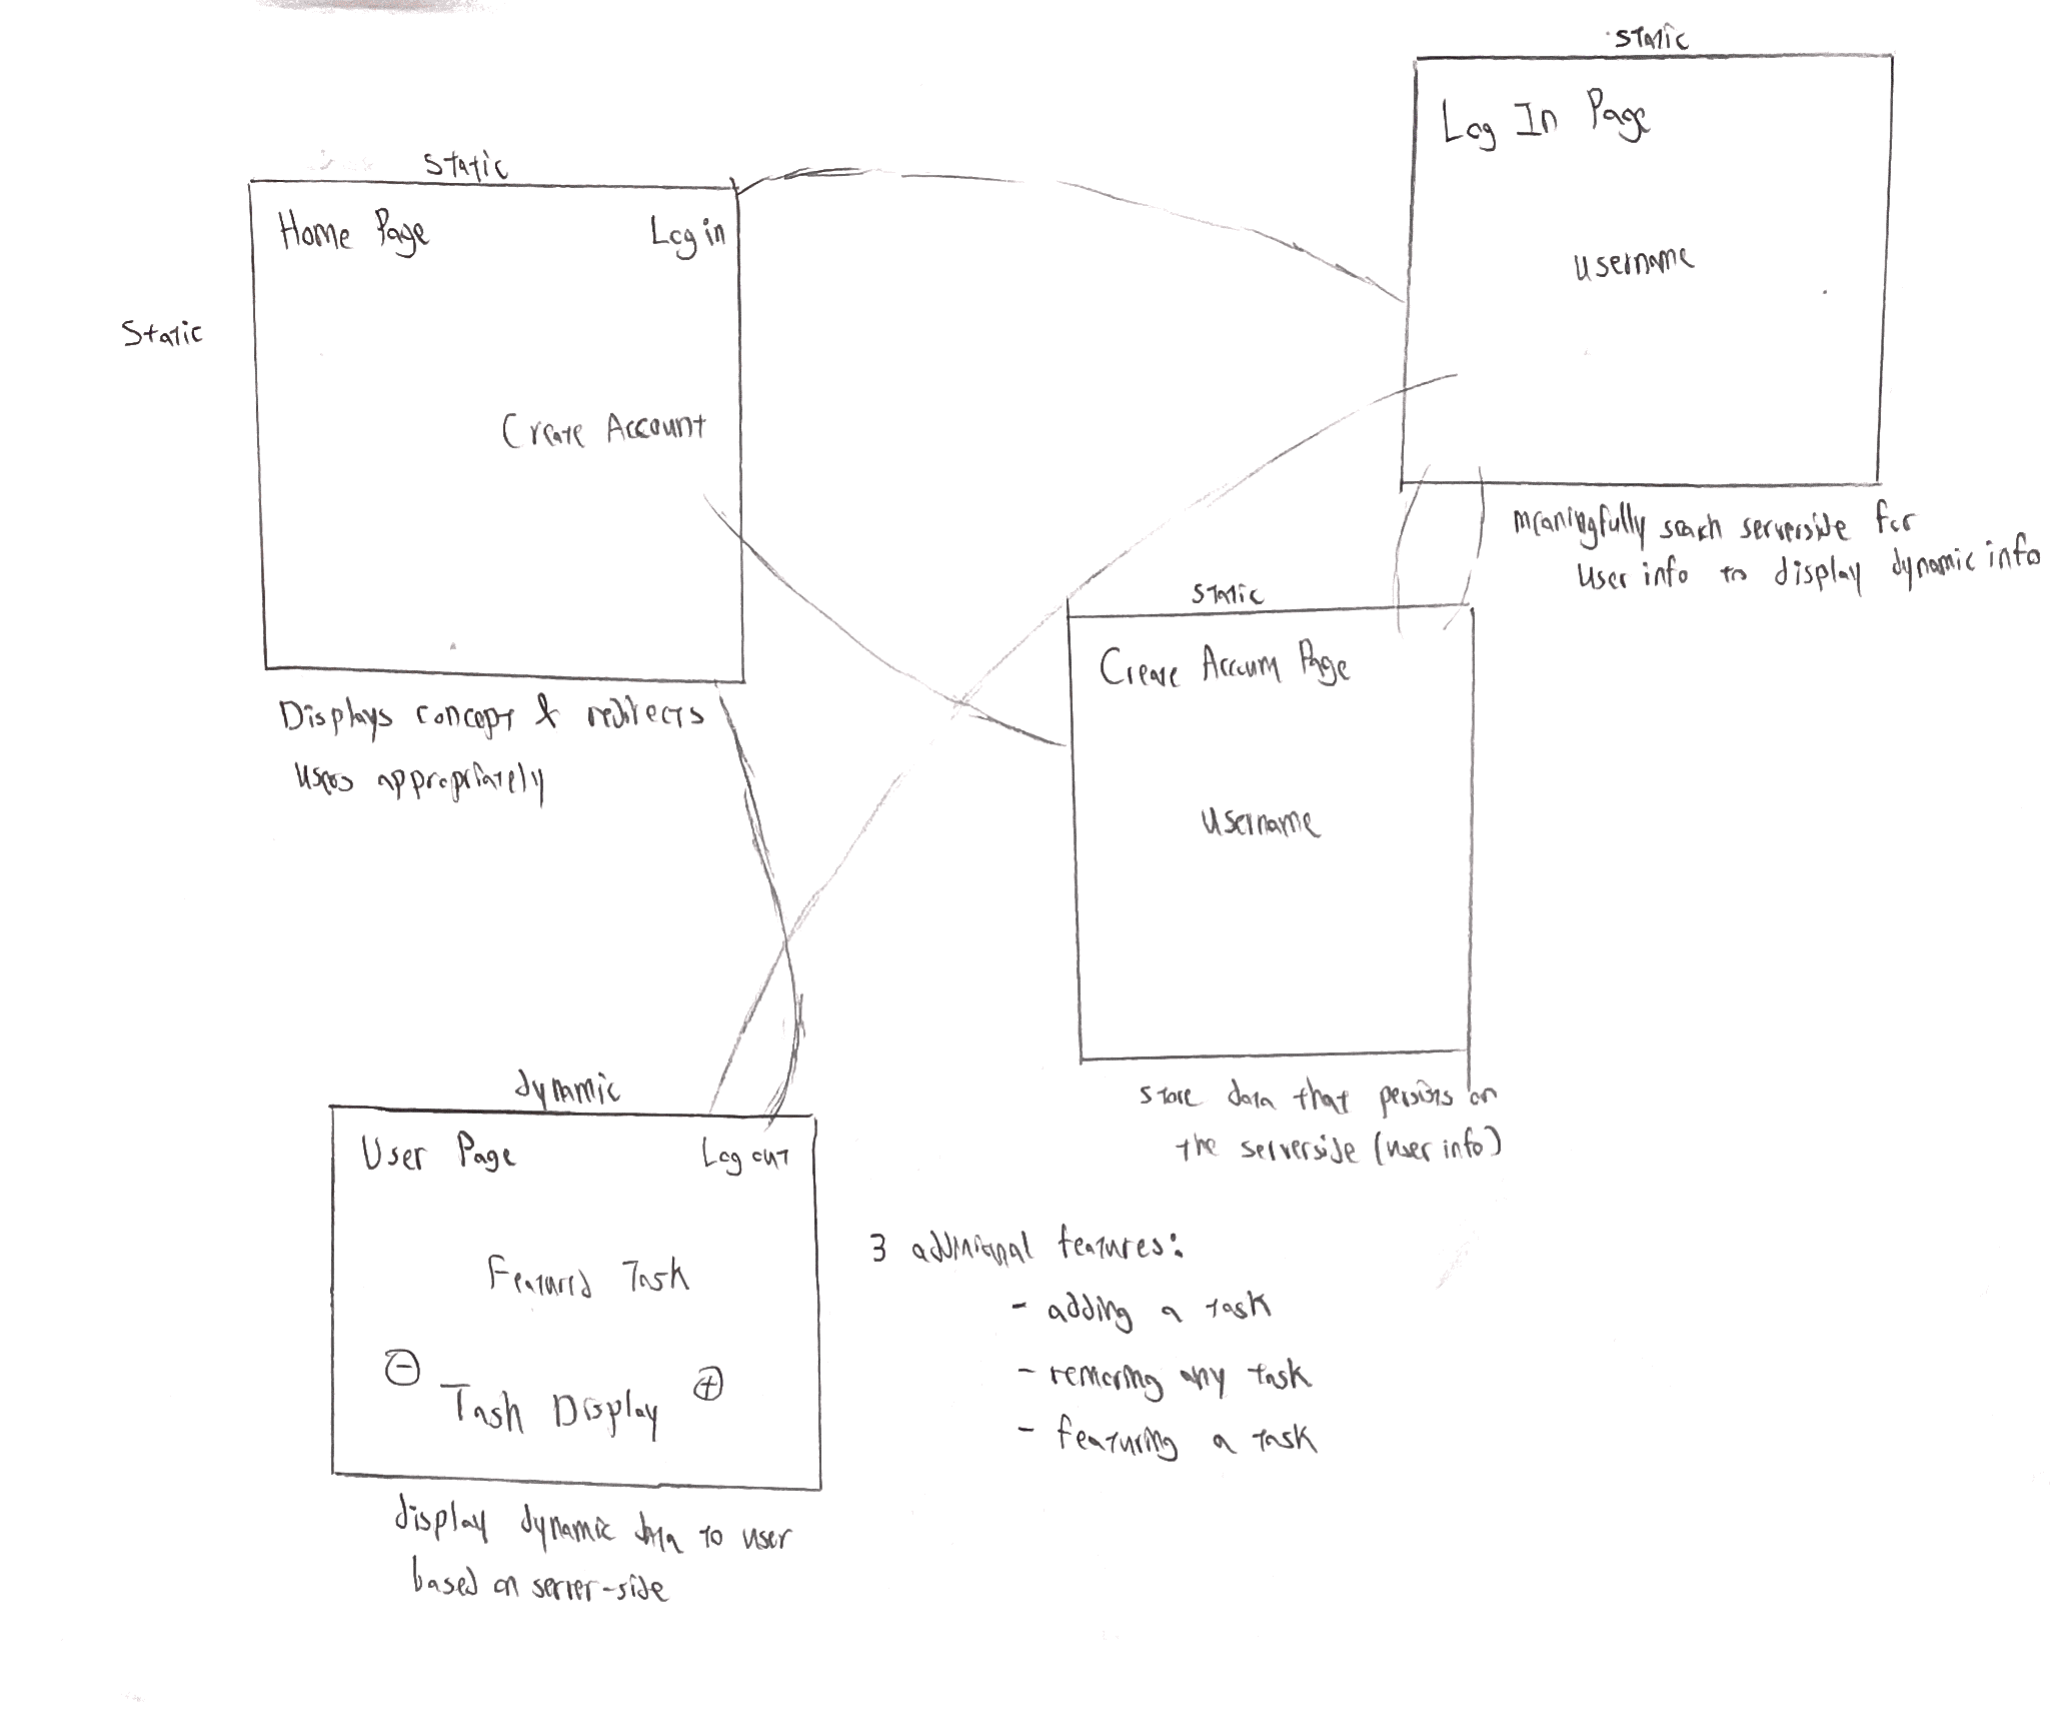
\includegraphics[width=0.75\textwidth]{illustration.png}
	\caption{System Design}
	\label{fig:design}
	\end{center}
\end{figure}

\tab In Figure \ref{fig:design}, you will see an overview of the interactions between different parts of the user-end structure. The requirements are met as follows:

\begin{enumerate}
	\item \textbf{General Requirements}
	\begin{enumerate}
		\item \emph{User can upload data to server that persists}: The user uploads their log-in information to the user, which is stored alongside the tasks associated with that user.
		\item \emph{User can meaningfully search through server-side data}: The user can input their log-in information in order to get access to their stored tasks.
		\item \emph{Dynamic data from server displayed to user}: Their stored tasks are presented to the user from the server and updated in real-time with their alterations.
	\end{enumerate}
	\item \textbf{Additional Features}
	\begin{enumerate}
			\item \emph{User can add new tasks}: User has the ability to add tasks to their task list, which are stored server-side.
		\item \emph{User can remove any particular task}: User has the ability to remove to remove any particular task from their task list, which will be updated server-side, refreshing their display.
		\item \emph{User can feature a task}: User has the ability to feature any particular task to take a dominant position on their display.
	\end{enumerate}
\end{enumerate}

\tab As such, we believe the project meets the general outline and requirements posed. Next up, our schedule to complete the project by the end of the term.
\end{document}